\documentclass[11pt,a4paper]{article}
\usepackage[utf8]{inputenc}
\usepackage[german]{babel}
\usepackage{amsmath}
\usepackage{amsfonts}
\usepackage{amssymb}
\usepackage{graphicx}
\usepackage[left=2cm,right=2cm,top=2cm,bottom=2cm]{geometry}
\author{Ward Schodts}

% Voor frames
\usepackage{mdframed}
% Voor kleuren
\usepackage{xcolor}

\definecolor{solarback}{HTML}{d9d9d9}
\definecolor{solarfront}{HTML}{000000}
\mdfdefinestyle{de}{linewidth=0pt,backgroundcolor=solarback,fontcolor=solarfront}
\newenvironment{de}[1]
{\begin{mdframed}[style=de]\begin{mydef}{\textbf{#1:}}\\} 
{\end{mydef}\end{mdframed}}
\newtheorem{mydef}{Definition}
\usepackage{float}

\newcommand{\tabitem}{~~\llap{\textbullet}~~}

\usepackage{array}
\newcolumntype{P}[1]{>{\centering\arraybackslash}p{#1}}

% Set graphics path

\graphicspath{{figures/}}
\usepackage{graphicx}
\usepackage{caption}
\usepackage{subcaption}

\begin{document}
\section{Was ist Projektmanagement?}
\subsection{Projekt}

\begin{de}{Projekt (DIN)}
Vorhaben, das im wesentlichen durch  Einmaligkeit der Bedingungen in ihrer Gesamtheit gekennzeichnet ist, wie z.B.:
\begin{itemize}
\setlength\itemsep{0em}
\item Zielvorgabe,
\item zeitlich, finanzielle oder andere Begrenzungen,
\item Abgrenzungen gegenüber anderen Vorhaben,
\item projektspezifische Organisation.
\end{itemize}

\end{de}

\begin{de}{Projekt (allgemein)}
Ein Projekt ist eine besondere, umfangreiche und zeitlich begrenzte
Aufgabe von relativer Neuartigkeit mit hohem Schwierigkeitsgrad und
Risiko, die in der Regel enge fachübergreifende Zusammenarbeit aller
Beteiligten fordert.
\end{de}

\begin{table}[H]
\def\arraystretch{1.2}
\centering
\begin{tabular}{|p{0.2\textwidth}|p{0.7\textwidth}|}

\hline
\textbf{Kriterium} & \textbf{Beschreibung} \\

\hline
Zeitliche Befristung & 
\tabitem Festgelegter Anfangs- und Endzeitpunkt
\\
\hline
Neuartigkeit &
\vspace{-\topsep}
\begin{itemize}
\itemsep0em
\setlength{\itemindent}{-1.3em}
\item Keine sich wiederholenden Routinevorgänge
\item Neue Aufgabestellung mit besonderer Herausforderung
\end{itemize}
\\

\hline
Einmaligkeit &
\vspace{-\topsep}
\begin{itemize}
\itemsep0em
\setlength{\itemindent}{-1.3em}
\item Insgesamt einmaliges Vorhaben
\item Einzelne Aktivitäten innerhalb des Vorhabens können sich jedoch wiederholen
\end{itemize}\\

\hline
Größe & 
\tabitem Umfang müss Einrichtung eines Projektes und einer Projektorganisation rechtfertigen\\
\hline
Komplexität und Zusammenarbeit &
\vspace{-\topsep}
\begin{itemize}
\itemsep0em
\setlength{\itemindent}{-1.3em}
\item Verschiedene untereinander abhänge Teilaufgaben
\item Hoher Abstimmungsbedarf
\item Fächerübergreifende Zusammenarbeit
\end{itemize}\\

\hline
\end{tabular}

\caption{Kriterien für Projekte}
\end{table}

\begin{table}[H]
\centering
\def\arraystretch{1.4}
\begin{tabular}{|P{0.4\textwidth}|P{0.4\textwidth}|}
\hline
\textbf{Routine-Aufgaben} & \textbf{Projekte}\\
wiederholende Tätigkeiten & einmalige Tätigkeiten\\
standardisierbare Tätigkeiten & individuelle Tätigkeiten\\
trainierbare Tätigkeiten & ``do it right the first time'' Anspruch\\
reproduzierbare Ergebnisse & selten reproduzierbare Ergebnisse\\
systematische Fehler leicht erkennbar  & systematische Fehler schwer erkennbar\\
kontinuierbare Verbesserung möglich & sofortige Korrektur notwendig\\
meist abteilungsspezifische Abwicklung & meis interdisziplinäre Abwicklung\\
meist statische Randbedingungen & meist dynamische Randbedingungen\\
\hline
\end{tabular}
\caption{Differenz zwischen Routine und Projekt}
\end{table}

\subsubsection*{Übung}
Schau die Übungsaufgabe (Welche Vorhaben sind Projekt?) noch mal an!
\subsection{Projektmanagement}

\begin{de}{Projektmangement (DIN)}
Gesamtheit von Führungsaufgaben, -organisation, -techniken und
–mittel für die Abwicklung eines Projektes.
\end{de}

\begin{de}{Projektmanagement (allgemein)}
Projektmanagement ist eine Führungskonzeption für direkte
fachübergreifende Koordination von Planung, Entscheidung,
Realisierung, Überwachung und Steuerung bei der Abwicklung
interdisziplinärer Aufgabenstellungen.
\end{de}

\section{Organisation des Projektmanagements}

\subsection{Organisationsstrukturen}

\begin{figure}[H]
	\centering
	\begin{subfigure}{0.45\textwidth}
		\caption*{Hierarchisches Organisationssystem:}
		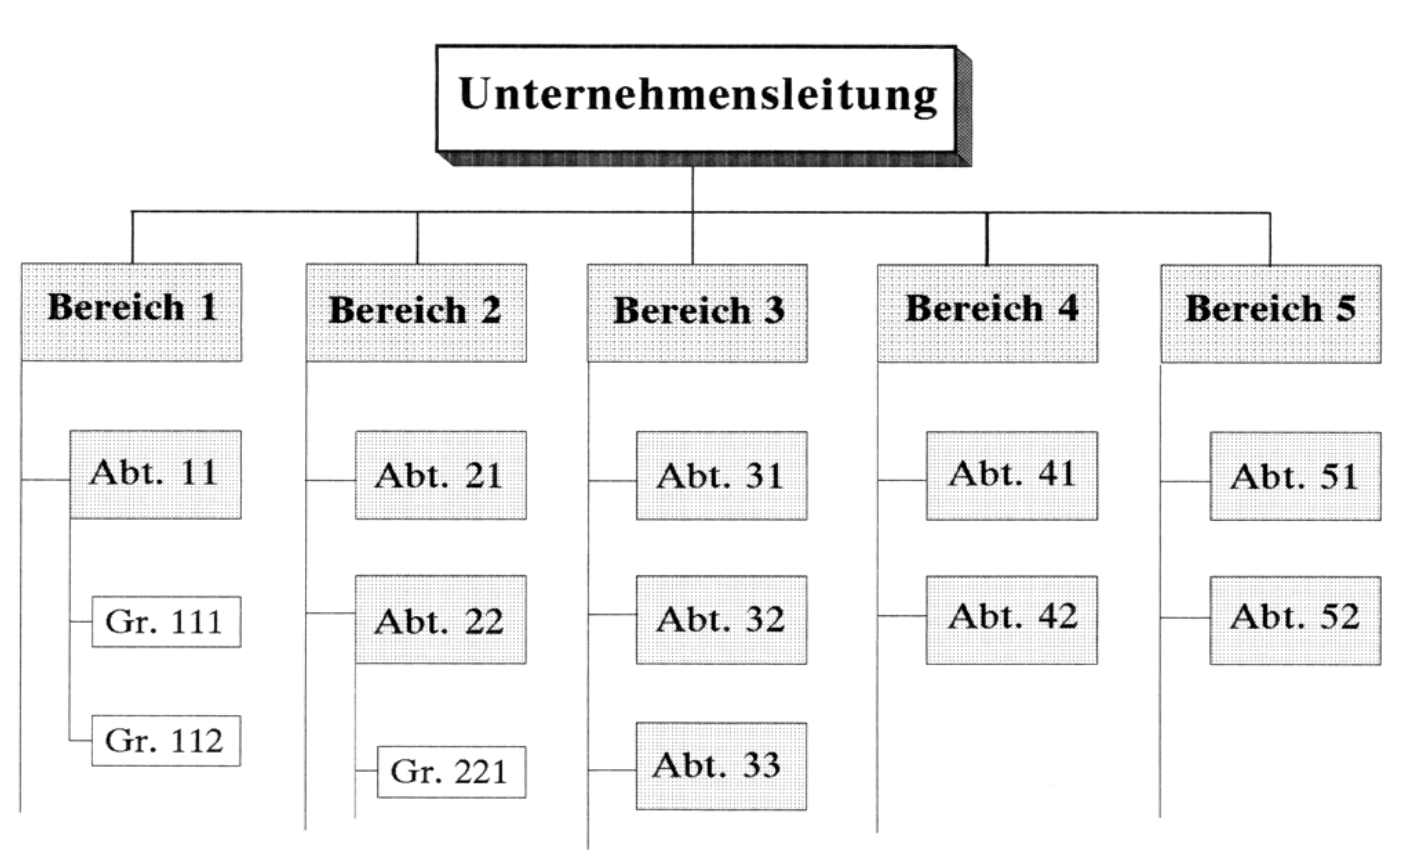
\includegraphics[width=\textwidth]{hierarchisches}
	\end{subfigure}
	~
	\begin{subfigure}{0.45\textwidth}
		\caption*{Funktionale Organisationsstruktur:}
		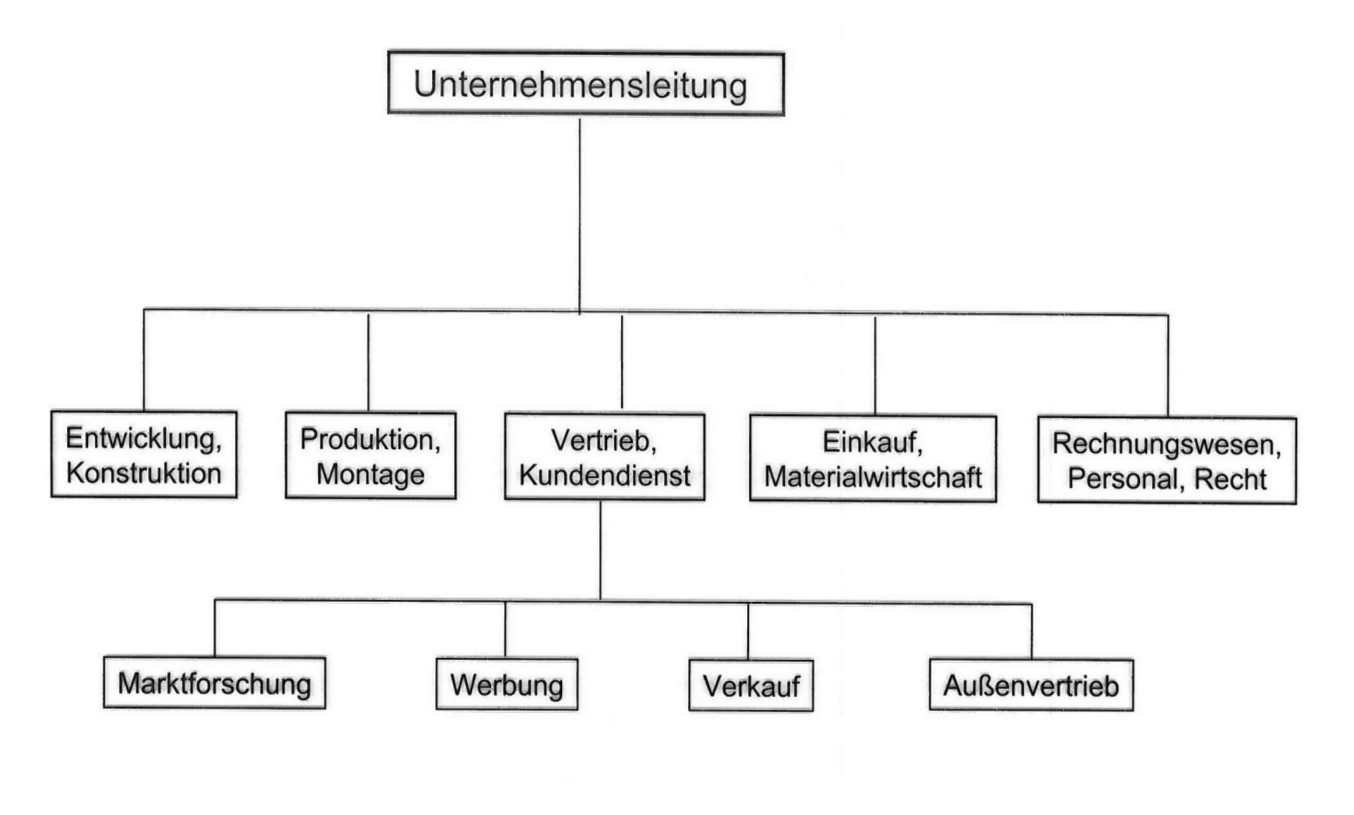
\includegraphics[width=\textwidth]{funktionale}
	\end{subfigure}
	\par\bigskip
	\par\bigskip
	\begin{subfigure}{0.45\textwidth}
		\caption*{Spartenorganisation:}
		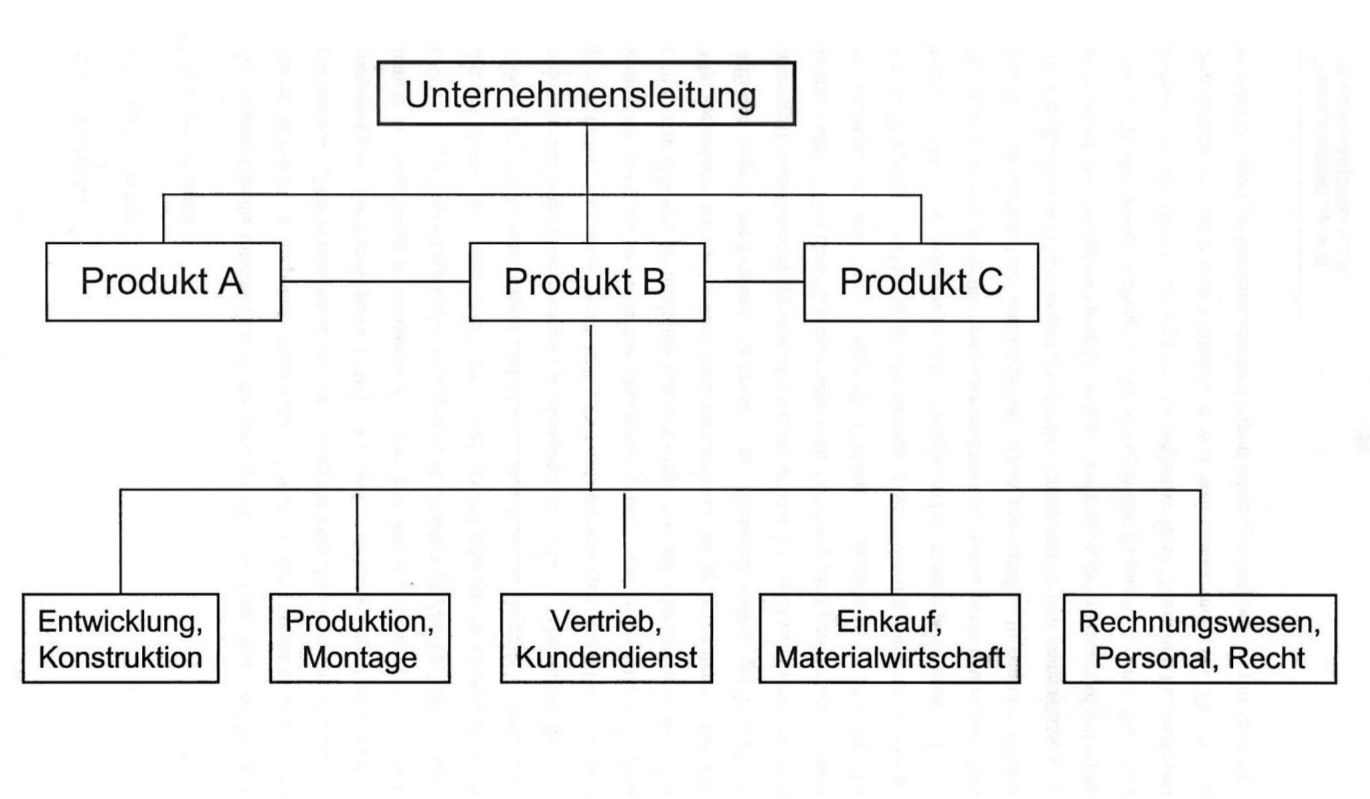
\includegraphics[width=\textwidth]{sparten}
	\end{subfigure}
	~
	\begin{subfigure}{0.45\textwidth}
		\caption*{Gemischte Organisation (Produkt- und fachbereiche):}
		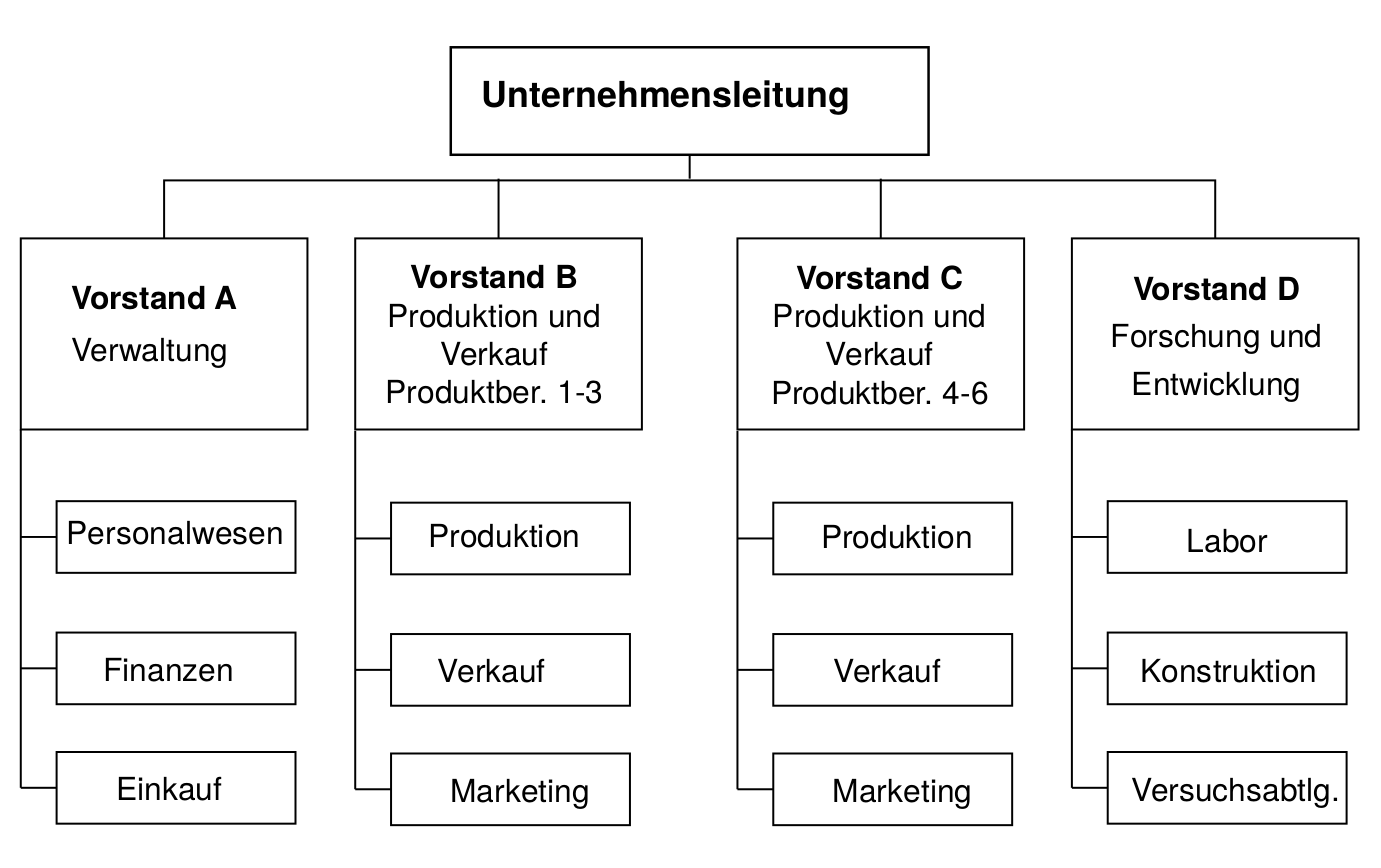
\includegraphics[width=\textwidth]{gemischte}
	\end{subfigure}
	
	\begin{subfigure}{0.5\textwidth}
		\caption*{Matrix-Organisation:}
		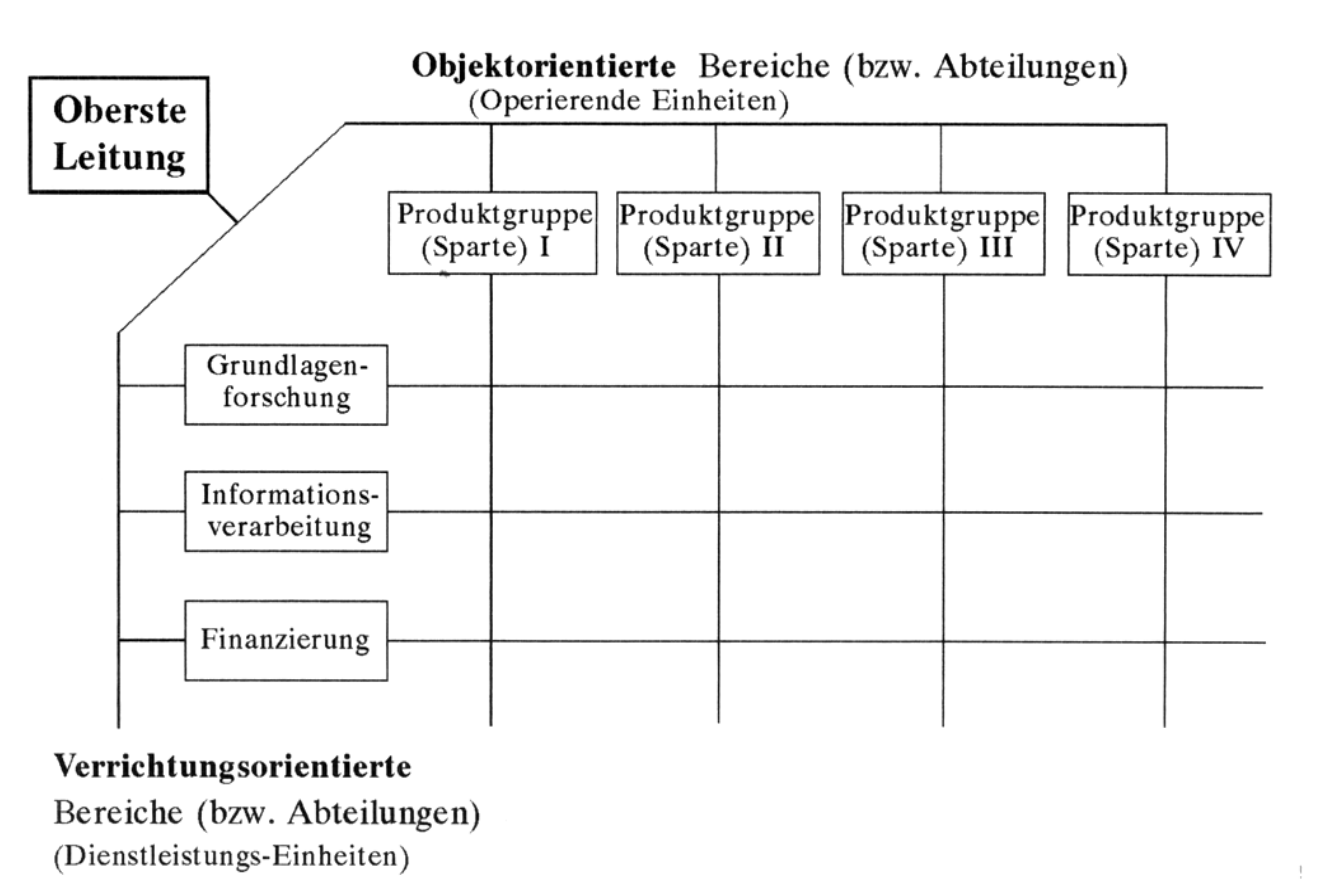
\includegraphics[width=\textwidth]{matrixorganisation}
	\end{subfigure}
\end{figure}

\begin{table}[H]
\centering
\def\arraystretch{1.4}
\begin{tabular}{|P{0.4\textwidth}|P{0.4\textwidth}|}
\hline
\textbf{Zentralisierung} & \textbf{Dezentralisierung}\\
\hline
\hline
Alle Vollmachten liegen bei der Unternehmensleitung & Delegation von Entscheidungen (Entscheidungen vor Ort)\\
\hline
Einheitliche Strategien, Prozeduren und Entscheidungen & Entlastung des Topmanagements\\

\hline
Minimierung der Duplikation von Funktionen & Entwicklung von Generalisten\\
\hline
Reduzierung der Gefahr, dass sich Firmenaktivitäten verselbständigen & Förderung der Zusammenarbeit (Teamgeist)\\
\hline
Umfangreiche Kontroll- und Koordinationsprozeduren nicht erforderlich & Produktspezialisierung\\
\hline
Direkter Einfluss des Topmanagement-Teams auf alle betriebliche Belange & Höhere Effizienz des Managements durch größere Nähe am Schauplatz\\
\hline
\end{tabular}
\caption{Wichtige vorteile der Zentralisierung und Dezentralisierung}
\end{table}

\subsection{Projektmanagement-Arten}
\subsubsection{Reines Projektmanagement}
\begin{minipage}[t]{0.5\textwidth}
	\subsubsection*{Vorteile:}

	\begin{itemize}
	\itemsep0em
		\item Straffe Projektleitung
		\item Klare eindeutige Projektverantwortung
		\item Einheit des Auftrags-Empfangs (Aufgabe \& Kompetenz)
	\end{itemize}
	\subsubsection*{Nachteile:}

	\begin{itemize}
	\itemsep0em
		\item Starre Organisationsform
		\item Hohe Gemeinkosten
		\item Eingliederung zeitlich begrenzter Spezialistentätigkeiten
	\end{itemize}
\end{minipage}
\hspace{0.5cm}
\begin{minipage}[t]{0.45\textwidth}
	\subsubsection*{Struktur:}
	\begin{figure}[H]
	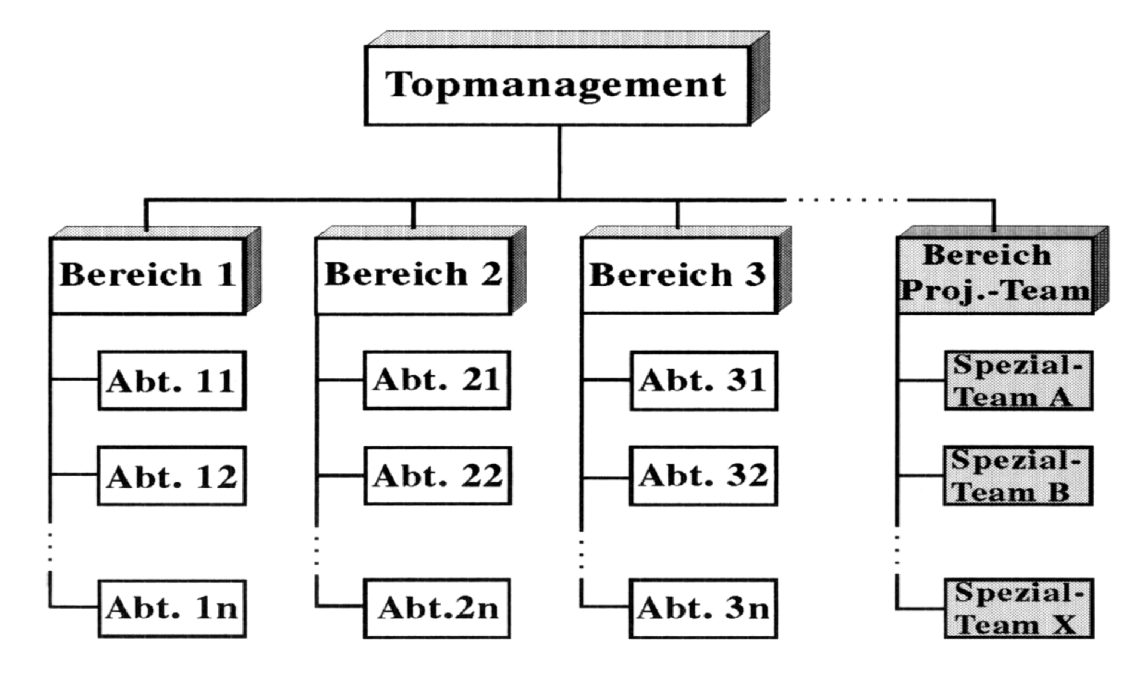
\includegraphics[width=\textwidth]{reines}
	\end{figure}
\end{minipage}
\vspace{1cm}

\subsubsection{Projektmanagement als Stabsfunktion (Einfluss-Projektmanagement)}
\begin{minipage}[t]{0.5\textwidth}
	\subsubsection*{Vorteile:}

	\begin{itemize}
	\itemsep0em
		\item Eingliederung des Projektteams ohne größere organisatorische Eingriffe möglich
		\item Flexibler Personaleinsatz
		\item Relativ gute Nutzung der Personalkapazitäten
	\end{itemize}
	\subsubsection*{Nachteile:}

	\begin{itemize}
	\itemsep0em
		\item Fehlende Weisungsbefugnis
		\item Der Projektleiter hat keine umfassende Projektverantwortung
	\end{itemize}
\end{minipage}
\hspace{0.5cm}
\begin{minipage}[t]{0.45\textwidth}
	\subsubsection*{Struktur:}

	\begin{figure}[H]
	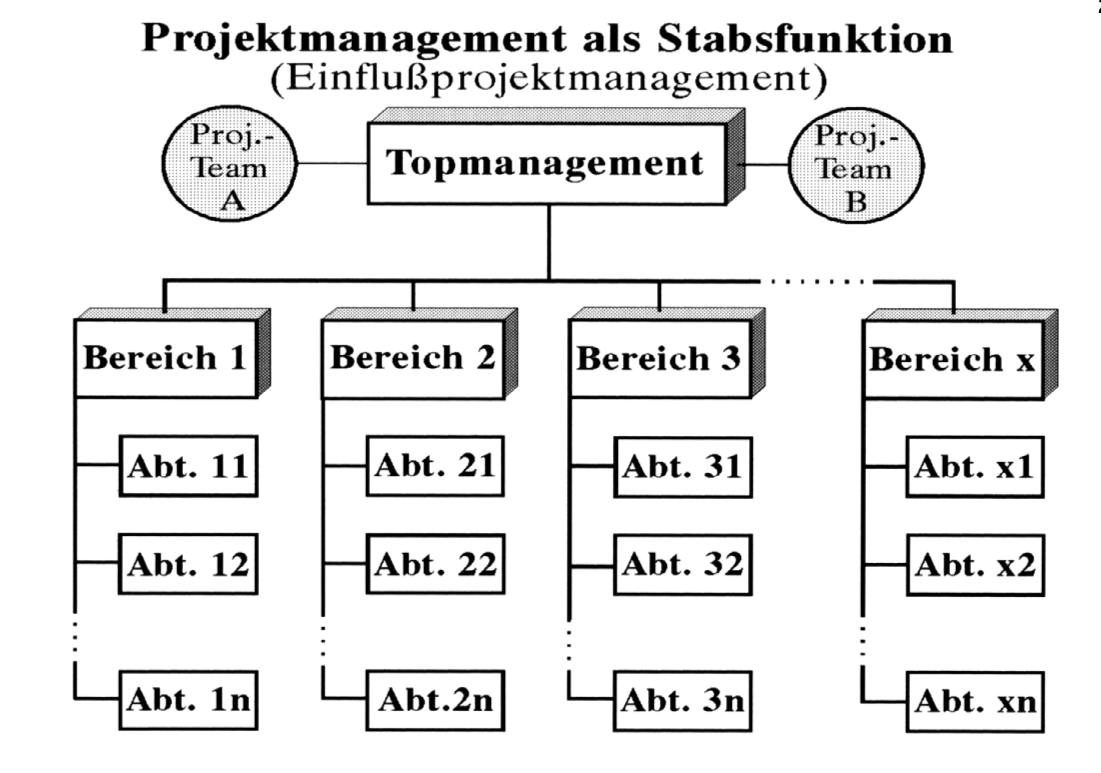
\includegraphics[width=0.95\textwidth]{stabsfunktion}
	\end{figure}
\end{minipage}

\vspace{1cm}
\subsubsection{Matrix-Projektmanagement}
\begin{minipage}[c]{0.5\textwidth}
	\subsubsection*{Vorteile:}

	\begin{itemize}
	\itemsep0em
		\item Flexible Eingliederung der Projektmitarbeiter
		\item Fachverantwortung des Projektleiters
	\end{itemize}
	\subsubsection*{Nachteile:}

	\begin{itemize}
	\itemsep0em
		\item Problematische Kompetenzabgrenzung
		\item Konflikte (zwischen ``Projekt'' und ``Linie'')
	\end{itemize}
\end{minipage}
\begin{minipage}[c]{0.45\textwidth}
	\subsubsection*{Struktur:}

	\begin{figure}[H]
	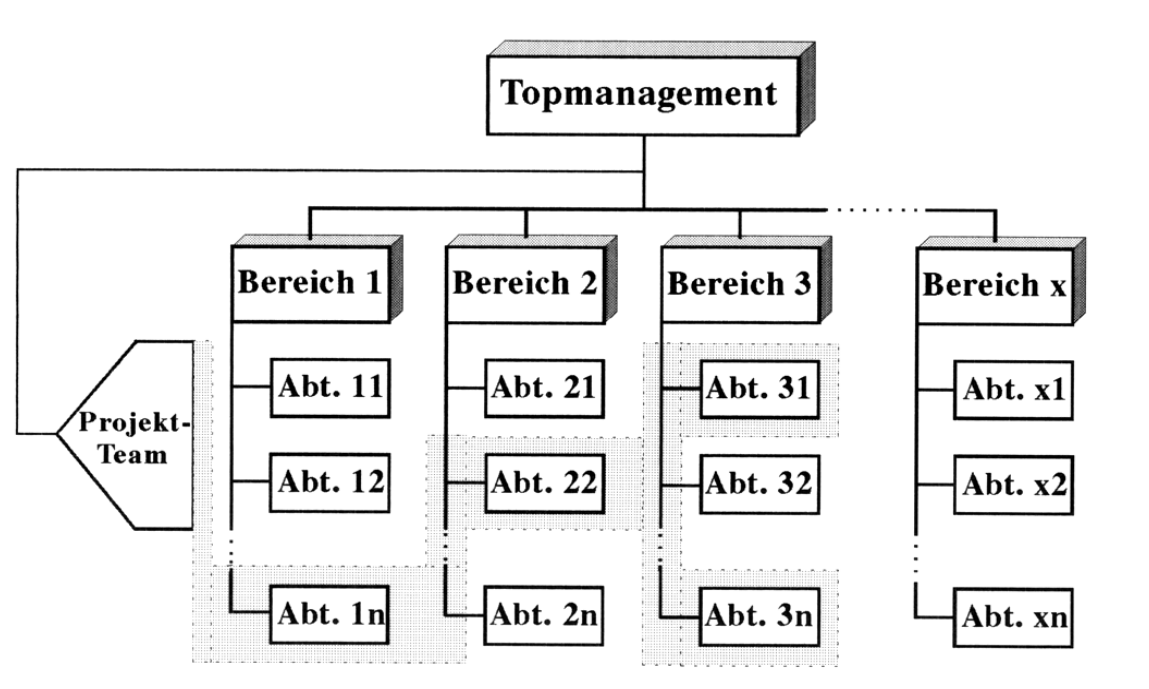
\includegraphics[width=\textwidth]{matrix1}
	\end{figure}
	
	\begin{figure}[H]
	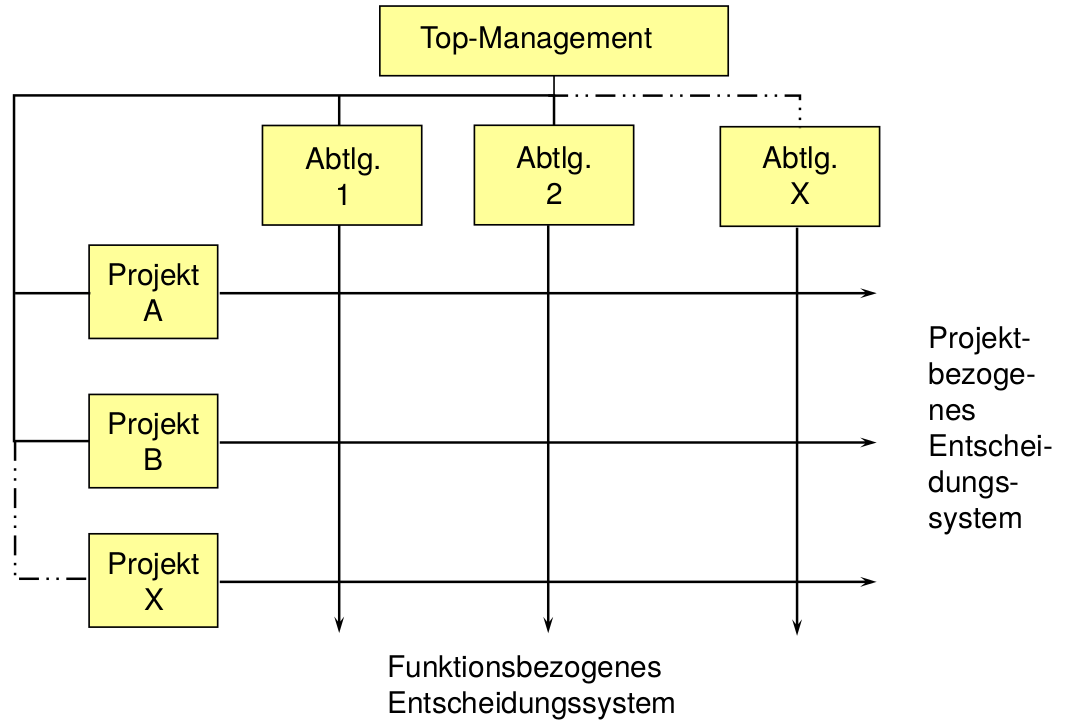
\includegraphics[width=\textwidth]{matrix2}
	\end{figure}
\end{minipage}

\vspace{1cm}

\subsubsection{Übersicht}

\begin{figure}[H]
	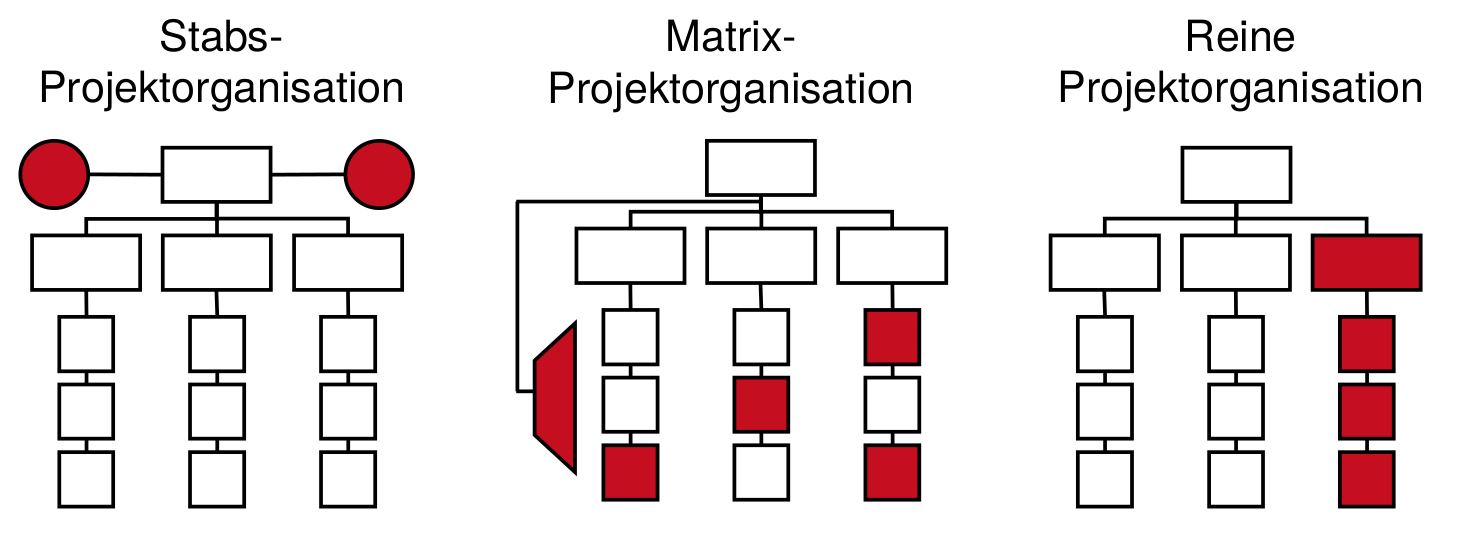
\includegraphics[width=\textwidth]{projektorganisation}
\end{figure}

\subsubsection{Empfehlungen für die Organisationsmodelle}
\begin{table}[H]
\centering
\def\arraystretch{1.2}
\begin{tabular}{|P{0.3\textwidth}|P{0.3\textwidth}|P{0.3\textwidth}|}
\hline 
	\textbf{Projektmanagement als Stabsfunktion} 
	
	& 
	
	\textbf{Matrix-Projektmanagement} 
	
	& 
	
	\textbf{Reines ProjektManagement}
	\\
\hline	
	\vspace{-\topsep}
	\begin{itemize}
	\itemsep0em
	\setlength{\itemindent}{-1.3em}
		\item Kleinere Projekte mit geringem Risiko und zeitlich nicht kritisch
		\item Erarbeitung von unternehmensweiten Kompromissen
		\item Nähe zum Top-Management, welches Bedeutung und Einflussnahme zeigt
	\end{itemize}
	
	&
	
	\vspace{-\topsep}
	\begin{itemize}
	\itemsep0em
	\setlength{\itemindent}{-1.3em}
		\item Hoher Anzahl laufender Projekte mit starkem Abteilungsübergriff (Interdiszplinarität)
		\item Relativ ähnliche Projekte
	\end{itemize}
	
	&
	
	\vspace{-\topsep}
	\begin{itemize}
	\itemsep0em
	\setlength{\itemindent}{-1.3em}
		\item Komplexe, neuartige Projekte
		\item Hohe strategische Bedeutung und starken Zeitdruck
		\item Bei langfristigen Projekten
	\end{itemize}
	\\
\hline	
	

\end{tabular}
\end{table}

\subsection{Kriterien verschiedener Organisationsformen des Projektmanagements}

\begin{figure}[H]
	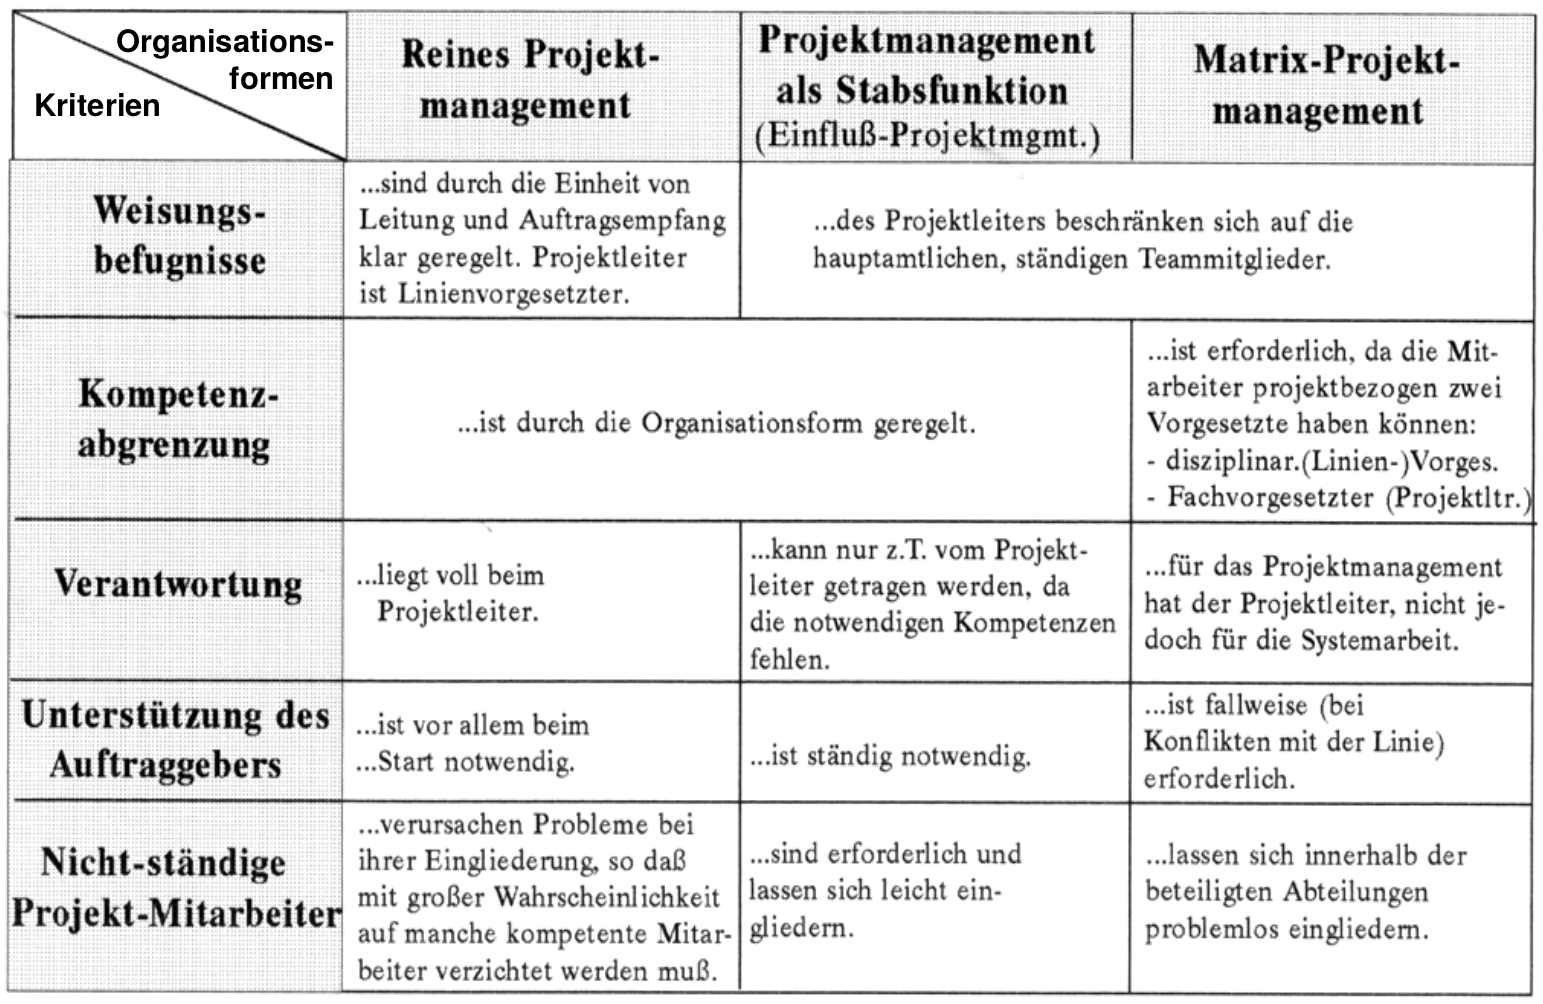
\includegraphics[width=\textwidth]{kriterien}
\end{figure}

\subsection{Literatur}
Kapitel 2.3.

\pagebreak

\section{Aufgaben des Projektmanagements}

\begin{figure}[H]
\centering
	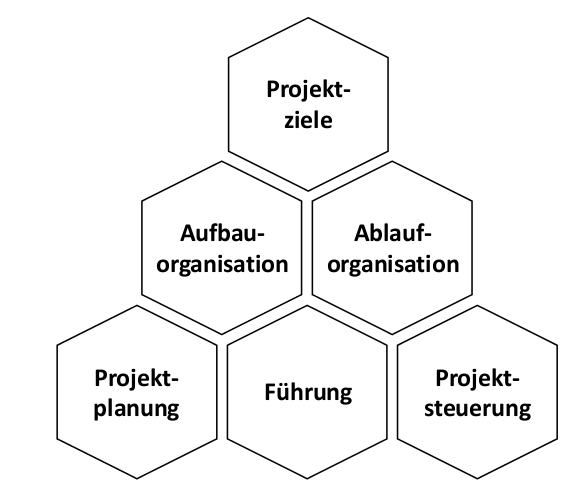
\includegraphics[width=0.36\textwidth]{hauptaufgaben}
\end{figure}


\subsection{Erfolgreiches Projektmanagements}

\subsubsection{Wesentliche Komponenten des Projektmanagements}
	\begin{figure}[H]
	\begin{enumerate}
	\itemsep0em
		\item \textbf{Klare Zielsetzung:} Sorgfältige Definition von klaren, eindeutigen, realistischen und von den Betroffenen akzeptierten Projektzielen und Zwischenzielen vor Inangriffnahme des Projektes.
		\item \textbf{Topmanagement-Engagement:} Projektunterstützung (einschl. Bereitstellung der erforderlichen Mittel
bzw.Kapazitäten) durch Topmanagement (Unternehmensleitung bzw.Auftrag
geber) und Führungskräfte der beteiligten Unternehmenseinheiten.
	
	\item \textbf{Teamarbeit/Kooperation:} Echte Teamarbeit (Teamgeist) innerhalb des Projektteams einschl. enger
Kooperation mit allen beteiligten Stellen.
\begin{center}
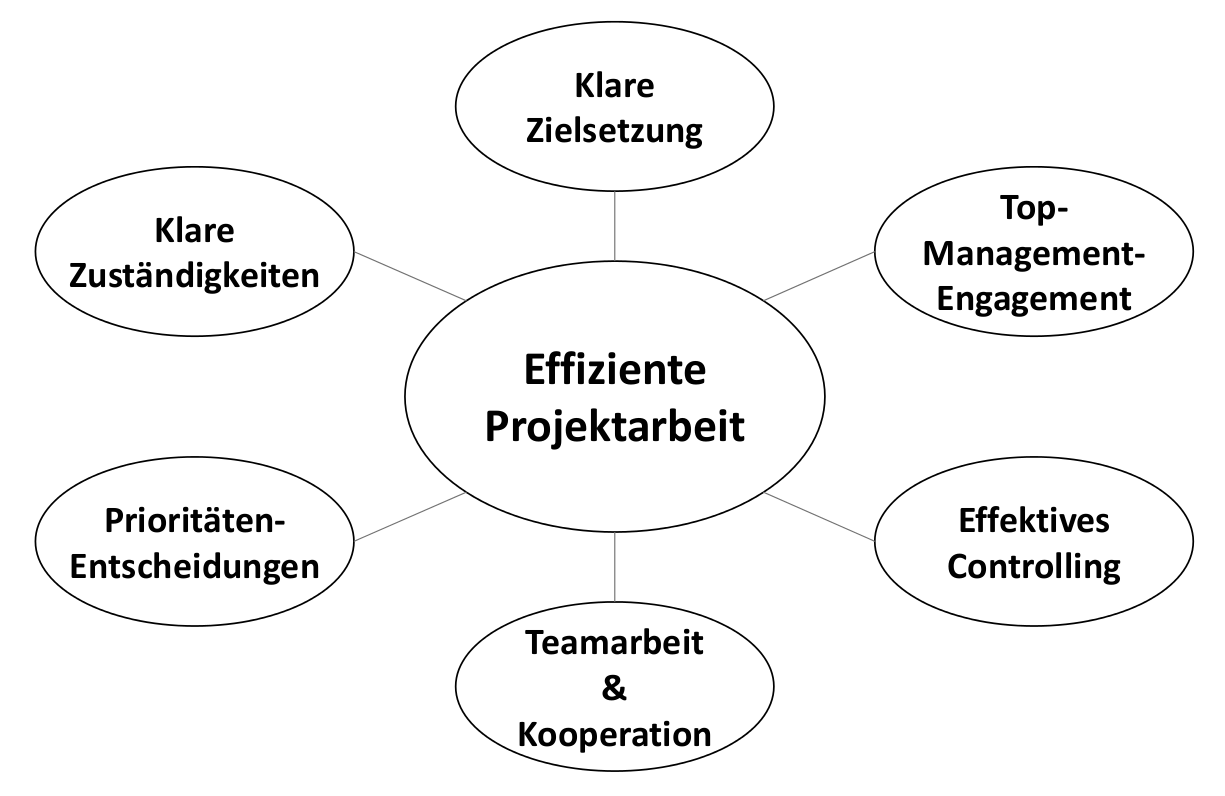
\includegraphics[width=0.5\textwidth]{effiizienteprojektarbeit}
\end{center}


	\item \textbf{Klare Zuständigkeiten:} Festlegung personifizierter Verantwortung und Kompetenz (einschl.
erforderlicher Befugnisse) mit dazugehöriger organisatorischer Regelung
und Überwachung.

	\item \textbf{Effektives Controlling:} Laufende Planung, Überwachung und Steuerung von Leistungsumfang
(Quantität \& Qualität), Zeit, Kosten und Kapazitäten.

	\item \textbf{Prioritäten-Entscheidung:} Laufende Prioritätenfestlegung aller aktuellen Projekte und Aufgaben
vor allem für die Bewältigung von Kapazitätsengpaßstellen.
	\end{enumerate}
	\end{figure}

\subsubsection{Hauptaufgaben}
\textbf{Ziele:} Definition klarere, eindeutiger, erreichbarer und akzeptierter Zieleund Zwischenziele als Basis Aller aktivitäten.
\begin{figure}[H]
\centering
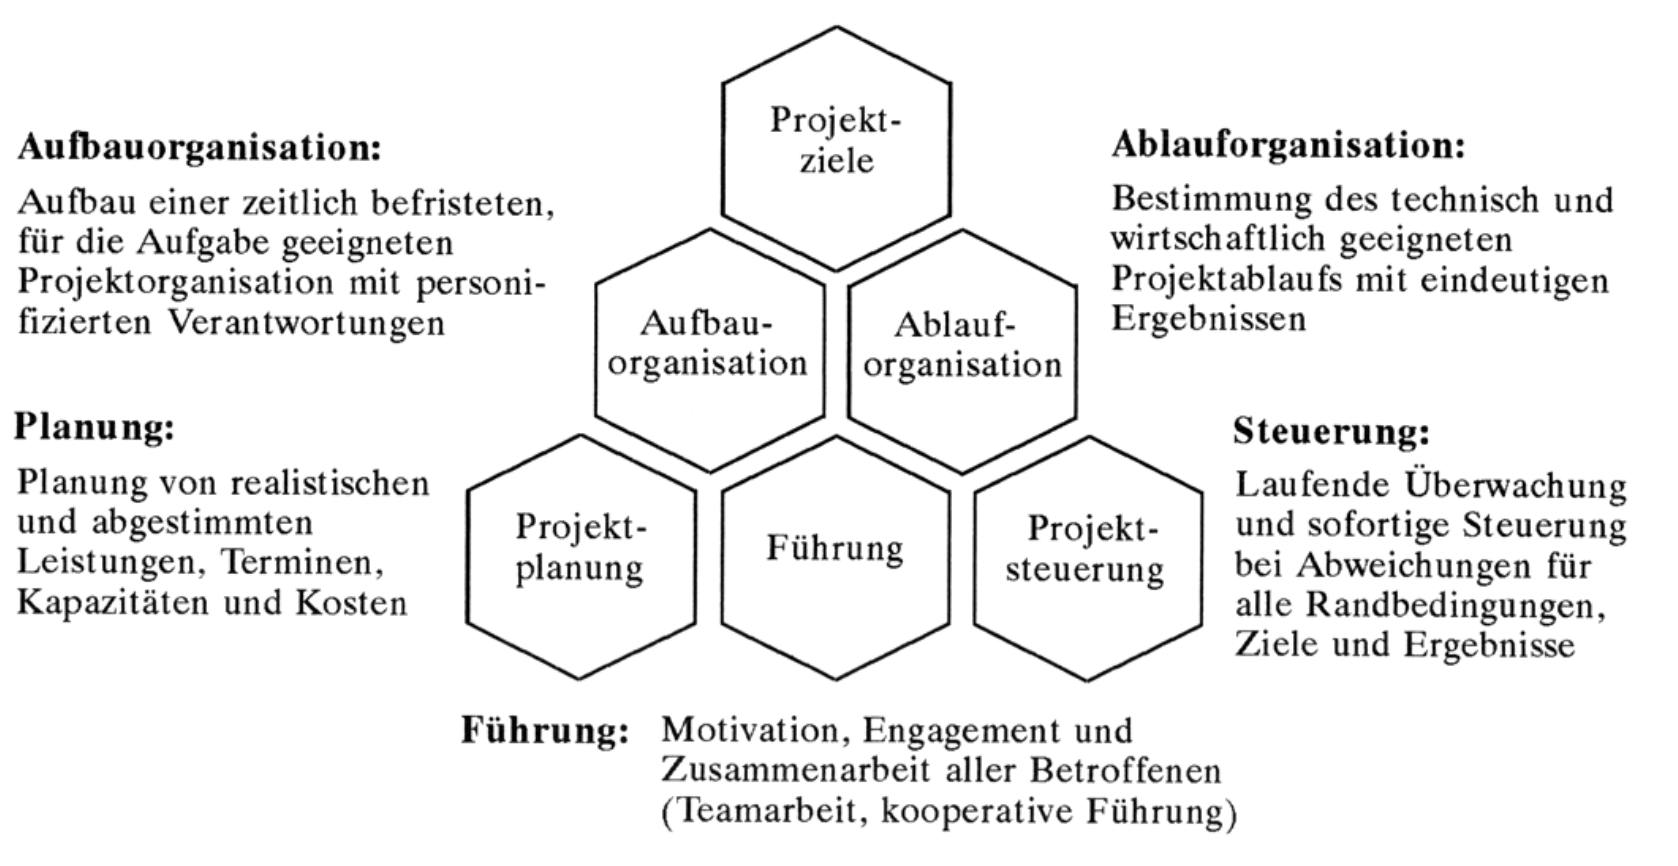
\includegraphics[width=0.95\textwidth]{hauptaufgabendesprojektmanagements}

\end{figure}


\subsubsection{Schwerpunkte für ein erfolgreiches Projektmanagement}

\begin{enumerate}
\item Beherrschung der \textbf{sachlichen} Aspekte für das Projektmanagement
(Organisation, Methoden, Hilfsmittel).

\item Beachtung \textbf{menschlicher Aspekte} beim Projektmanagement,
insbesondere bei der Teamarbeit und bei der Kooperation mit den
Mitwirkenden bzw. Betroffenen.

\item \textbf{Identifizierung} der verantwortlichen Leitung und der Führungskräfte
der betroffenen Einheiten sowie der Mitwirkenden \textbf{mit den Projektzielen}
und den Methoden des Projektmanagements;
d.h. der Erfolg des Projektmanagements hängt von der Kompetenz,
der strategischen Führung und der Unterstützung auf Leitungsebene
ab; denn Projektmanagement ist eine Art von „strategischer
Delegation“, bei der die leitenden Führungskräfte den Projekt-
managern die Kompetenz und die Verantwortung für Projektaufgaben
übertragen.
\end{enumerate}

\subsubsection{Voraussetzungen für den Erfolg eines Projektes}

\begin{enumerate}
\item Starke Einbindung des Auftraggebers bei Projektplanung
und -durchführung.

\item Eine umfassende Machbarkeitsstudie des Projektes während der
strategischen Planungsphase des Unternehmens.

\item Fortlaufende Projektplanung, -koordinierung und -überprüfung.

\item Teamarbeit, die sich aus der Konzentration auf eine klar
umrissene Zielsetzung ergibt.

\item Verpflichtung des Auftraggebers, technische Konstruktions-
entscheidungen, Projektmanagementzielsetzungen und moderne
Managementverfahren zu unterstützen.

\item Sicherstellung, dass die Prinzipien des Projektmanagements
allen Mitarbeitern des Projektteams und den am Projekt
Beteiligten – einschl. Führungskräften – bekannt sind.
\end{enumerate}

\subsection{Der Projektleiter}

\subsubsection{Aufgaben eines Projektleiters}
\begin{itemize}
\item Definition der Aufgabe und Planung eines Projektes, Aufwandschätzung,
Zeitschätzung (Netzplan)
\item Aufgabenverteilung, Abgrenzung der Teilgebiete
\item Festlegung von Methoden und Verfahren
\item Koordination - Projektteam
- Fachabteilungen
- externe Beratung
\item Überwachung von - Projektfortschritt/Leistungsumfang (Quantität/Qualität)
- Zeit (Termine)
- Kosten
- Änderungen (change control)
\item Erkennung von Engpässen und möglichen Risiken
\item Erarbeitung von Lösungsmöglichkeiten
\item Dokumentation und Berichtwesen
\item Beschaffung von Mitteln zur Realisierung des Projektes (HW, SW, Testzeit...)
\item Projektsteuerung und Zusammenarbeit mit dem Auftraggeber (Vertragstreue)
\end{itemize}

\subsubsection{Forderungen an einen Projektleiter}
\begin{figure}[H]
	\centering

	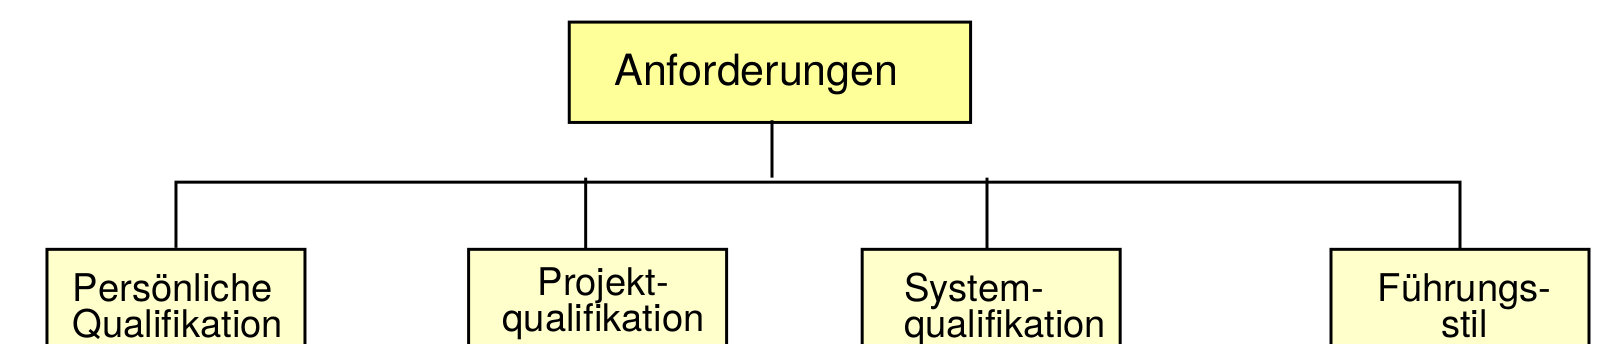
\includegraphics[width=\textwidth]{forderungen}

\end{figure}	

\textbf{Persönliche Qualifikation:} 
\begin{itemize}
\itemsep0em
	\item Teamgeist
	\item Initiative
	\item Kreativität
	\item Kontaktfähigkeit
	\item Durchsetzungsvermögen
\end{itemize}
\noindent
\textbf{Projektqualifikation:} beinhaltet Kenntnisse und Erfahrungen,
die sich auf die Organisationsmethoden
und -techniken beziehen.
\\
\\
\textbf{Systemqualifikation:} Sie beinhaltet alle Kenntnisse und
Funktion des Projektes. (z.B. Maschine,
Projektleiter sprechen können.
Chemieanlage, Kraftwerk, EDV-Systeme).
\\
\\
\textbf{Führungsstil:} der Projektleiter hat einen kooperativen Führungsstil:
\begin{itemize}
\item Der Mensch steht im Mittelpunk
\item Prinzip der offenen Tür.
\item Führung durch Überzeugung und Argumentation
\item ...
\end{itemize}
\subsection{Ziele}

\textbf{Organisatorische Ziele:}
\begin{itemize}
\item Entwicklung einer flexiblen projektorientierten Organisationsstruktur
mit eindeutiger Regelung der Kompetenzen, Informations- und Entscheidungswege.
\item Klarheit über den Projektablauf bei allen Beteiligten.
\item Sicherstellung der fachübergreifenden Kooperation.
\end{itemize}
\noindent
\textbf{Planungs-Ziele:}
\begin{itemize}
\item Beherrschung des Umfangs und der Komplexität durch inhaltliche Strukturierung.
\item Erzielung einer angemessenen Lastverteilung im Team.
\item Einhaltung von Zeit-, Kosten- und Kapazitätsplanungen.
\end{itemize}
\noindent
\textbf{Controlling-Ziele:}
\begin{itemize}

\item Frühzeitige Erkennung von Planabweichungen und deren zukünftigen Auswirkungen.
\item Aufzeigen von Handlungsalternativen bei Planabweichungen.

\item Dokumentation des Projektverlaufs zur Verwertung in zukünftigen Projekten.
\item Steigerung des Termin- und Kostenbewußtseins bei allen Projektbeteiligten.

\end{itemize}
\noindent
\textbf{Führungsziele:}
\begin{itemize}
\item Steigerung der Produktivität durch:
\begin{itemize}
\item Motivation des Projektteams
\item Konsensbildung durch Entscheidungsdokumentation
\item Erkennen und Lösen von Konfliktsituationen
\item Hohe Akzeptanz durch Anwender-Partizipation
\end{itemize}
\end{itemize}

\subsubsection{Formulierung von Zielen}
Zielen sollten:
\begin{itemize}
	\item SMART:
	\begin{itemize}
		\item \textbf{Spezifisch:} klar und eindeutig
		\item \textbf{Messbar:} wir können das auf eine Schale angeven (Begin mit endzustand vergeleichen)
		\item \textbf{angemessen:} redelijk, realistisch
		\item \textbf{Relevant:}  begrenzt in zeit, man weißt wenn es endet.
	\end{itemize}
	\item lösungsneutral formuliert sein. (do not say how it should be solved)
\end{itemize}

\subsubsection{Zielbeziehungen}

Es gibt drei verschiedene Zielbeziehungen:
\begin{itemize}
\item \textbf{Iterdependenzrelation:} Beeinflussung verschiedener Ziele untereinander: komplementär, konfliktär.
\item \textbf{Präferenzrelation:} Prioritäten von
konkurrierenden Zielen
\item \textbf{Instrumentalrelation:} Ziel-Mittel-Verhältnis von Zielen (the subtarget serves the upper target)
\end{itemize}

\section{Projektverantwortung}

\subsection{Projektsysteme in der Projektorganisation}
\textbf{Politisches Projektsystem:} = politisches Teilsystem des Projektmanagements, also Auftraggeber,
Steuerungsausschuß oder -ausschüsse.
\\
\\
\textbf{Administratives Projektsystem:} = administratives Teilsystem des Projektmanagements, also Projektleitung.
\\
\\
\textbf{Operatives Projektsystem:} = Projektdurchführung (Projektrealisierung).

\subsection{Kooperation}

\begin{figure}[H]
	\centering

	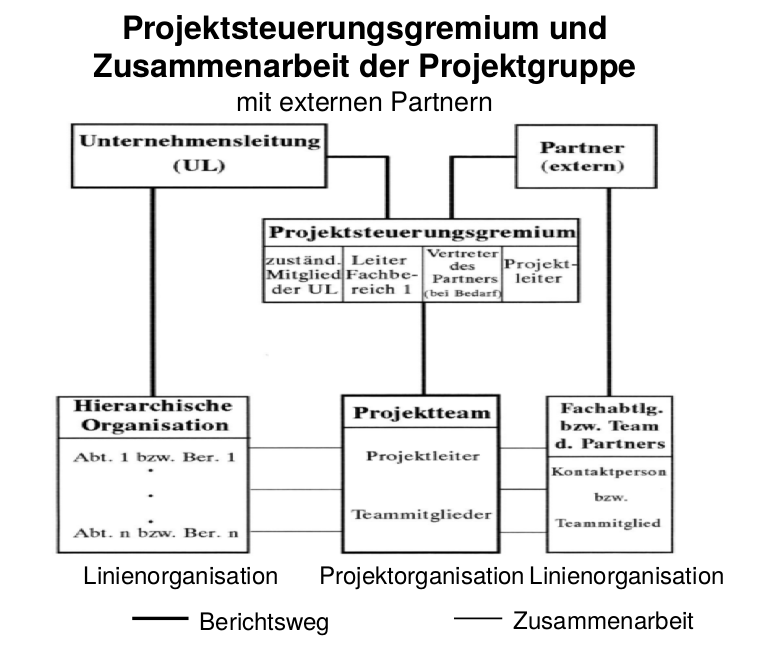
\includegraphics[width=0.66\textwidth]{ch4/projektgruppe}

\end{figure}	

\begin{figure}[H]
	\centering

	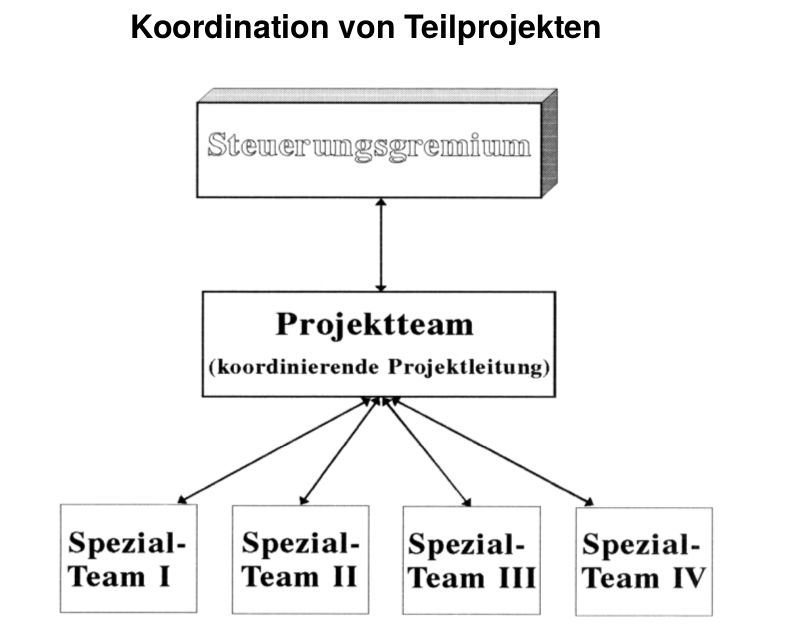
\includegraphics[width=0.66\textwidth]{ch4/teilprojekt}

\end{figure}	

\begin{figure}[H]
	\centering

	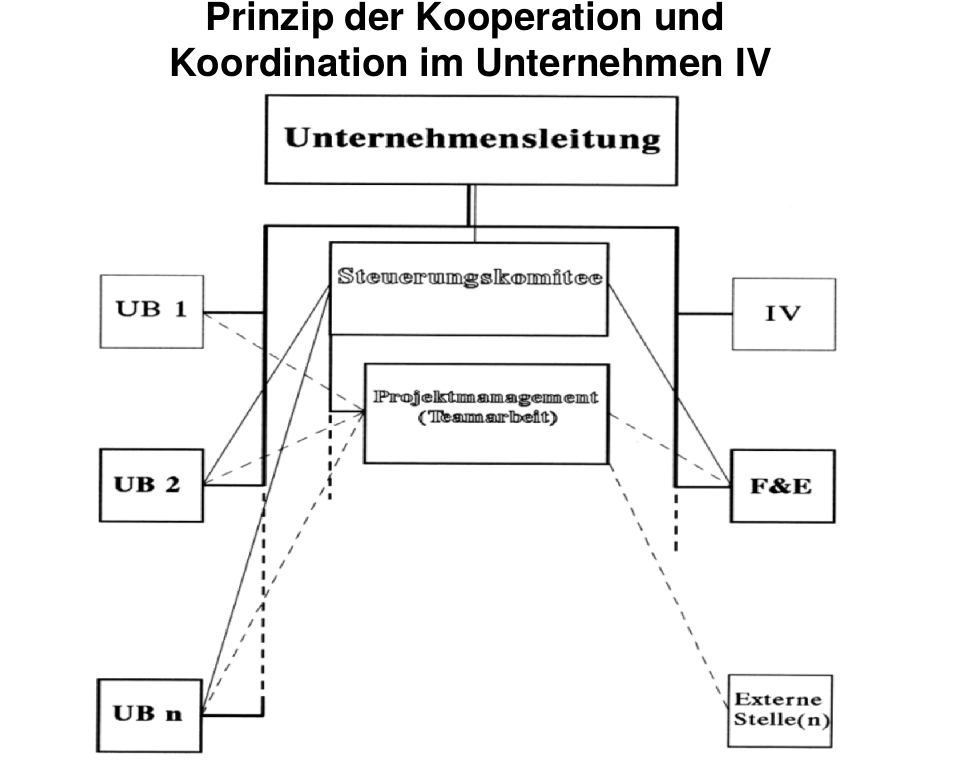
\includegraphics[width=0.66\textwidth]{ch4/kooperation}

\end{figure}	

\section{Das projektteam und seine Afugaben}

\begin{de}{Projektteam}
Ein Projektteam ist eine interdisziplinäre und hierarchieübergreifende Areitsgruppe, die in der Lage ist, eine bestimmte Aufgabe in Projektform zu lösen.
\end{de}
\textbf{Warum Teamarbeit?} Einwirkung verschiedener Fachdisziplinen auf komplexe Aufgabenstellungen

\begin{de}{Effizient arbeiten}
die Dinge richtig tun
(in Bezug auf Qualität, Kosten. Termine etc.)
\end{de}

\begin{de}{Effektiv arbeiten}
die richtigen Dinge tun
(in Bezug auf die Arbeitsschritte im Projektablauf,
Prioritäten gemäß Pflichtenheft vs. Änderungen
seitens Auftraggeber etc.)
\end{de}

\begin{de}{Kommunikation im Projektteam}
$$
N = \frac{n(n-1)}{2}
$$
\end{de}

\begin{de}{Soft skills}
weiche, das soziale Umfeld berücksichtigende Fähigkeiten:\\
\\
Tadellose Manieren, vorbildlicher Charakter, Planung von Einstieg und
Aufgabe (Ziel) sowie Beziehungs- und Rückkopplungsnetzwerk (Weg).
\end{de}

\begin{de}{Hard skills}
in Schule und Hochschule erworbene fachliche Fähigkeiten:\\
\\
Techn. und kaufm. Fachkönnen, Wissen in Theorie und Anwendung zur
Erarbeitung exzellenter Lösungen zunehmend schwierigerer Aufgaben.
\end{de}

Hard und Soft Skills worden zusammen angewendet auf 3 verschiedene Ebene:
\begin{itemize}
\item \textbf{Fachwissen:} Ein Mitarbeiter muss sein Fachkönnen und -wissen so
anwenden, daß die ihm aufgetragenen ``Dinge richtig'' erledigt werden.
\item \textbf{Organisationswissen:} Ein Vorgesetzter muß dafür Sorge tragen, daß die
``richtigen Dinge'' getan werden.
\item \textbf{Herrschaftswissen:} Ein Mitglied von Vorstand/Geschäftsführung muß
dafür sorgen, daß
\begin{itemize}
	\item im Unternehmen das notwendige Wissen, Können und Motivation
vorhanden sind, um die ``Dinge richtig'' auszuführen.
	\item bei allen Vorhaben (Projekten) klar definiert wird, was die ``richtigen
Dinge'' sind, die zum Wohle der Firma getan werden müssen.
\end{itemize}
\end{itemize}
\subsection{Art des Projektteams}
Projektteams können im Hinblick auf die Zahl und die
Person der Teammitglieder fix oder veränderbar sein.

\begin{itemize}
\item \textbf{Geschlossenes Projektteam:} bei dieser Art eines Projektteams ist geplant, dass vom Anfang bis zum
Ende die Mitarbeiter des Projektes gleich sind, sowohl hinsichtlich ihrer
Zahl als auch ihrer Person.

\item \textbf{Offenes Team:} die Zusammensetzung dieses Projektteams ändert sich im Laufe der
Projektabwicklung. Es werden für die einzelnen Phasen in der Projektarbeit
jeweils unterschiedliche Mitarbeiter und diese in unterschiedlicher Zahl
zur Projektarbeit eingesetzt.

\item \textbf{Externes Projektmanagement:} Der Auftraggeber lässt das Projekt ausschließlich durch betriebsfremde
Mitarbeiter planen, kontrollieren und ggf. auch realisieren. D.h. das Projekt-
team besteht nur aus betriebsexternen Mitgliedern.

\item \textbf{Internes Projektmanagement:} An dem Projekt sind ausschließlich eigene Mitarbeiter des Auftraggebers
beteiligt. D.h. das Team besteht nur aus betriebsinternen Mitgliedern.

\item \textbf{Gemischtes Projektmanagement:} Die Planung und Kontrolle eines Projektes liegt in den Händen eines Teams,
das aus externen und internen Mitgliedern gebildet wird.
\end{itemize}

\begin{figure}[H]
	\centering

	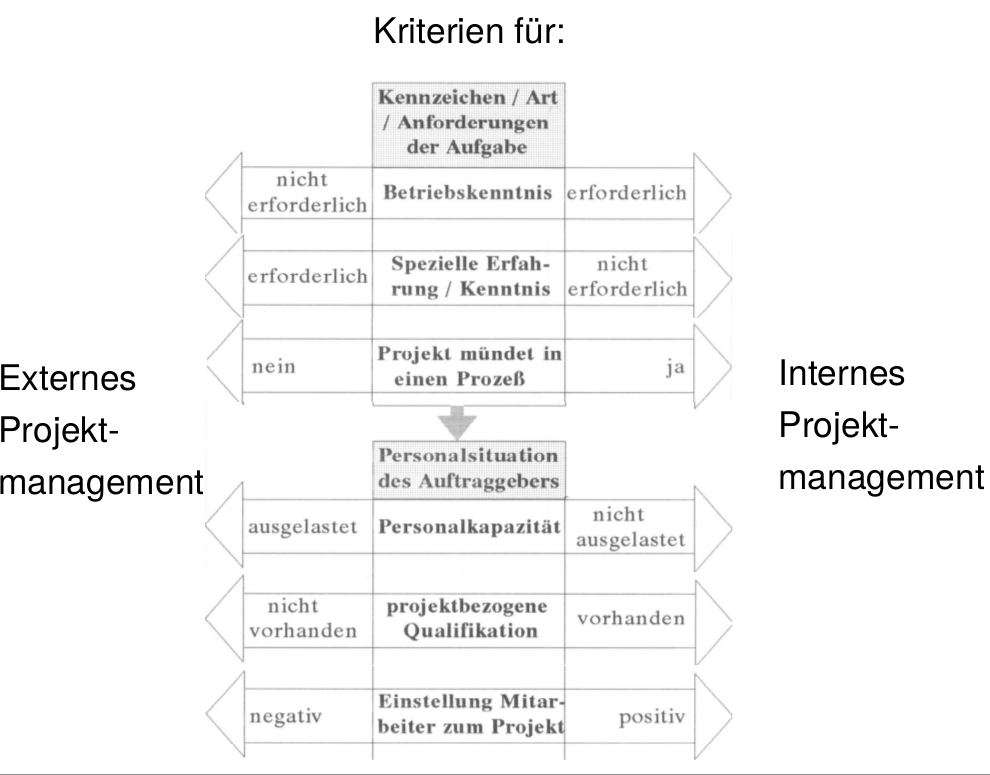
\includegraphics[width=0.66\textwidth]{ch5/kriterien}

\end{figure}	



\subsection{Aufgaben des Projektteams}
\textbf{Das Projektteam (bzw. die Projektleitung)}

\begin{itemize}
\item \textbf{plant} das ihm anvertraute Projekt im Detail und überwacht dessen Verlauf;
\item \textbf{koordiniert} die Zusammenarbeit aller beteiligten Stellen;
\item \textbf{informiert} die Unternehmens- bzw. Institutsleitung laufend über den Stand
des Projektes, insbesondere bei Schwierigkeiten;
\item \textbf{dokumentier} den Verlauf des Projektes in sachlicher, terminlicher und
finanzieller Hinsicht;
\item \textbf{führt} und \textbf{berät} alle am Projekt beteiligten Mitarbeiter
\item \textbf{bereitet} Entscheidungsunterlagen vor und führt Entscheidungen herbei.
\end{itemize}

\subsection{Kriterien für erfolgreiche Zusammenarbeit im Team}
\begin{enumerate}
\item Kommunikationsfähigkeit
\item Initiative, Engagement, Begeisterungsfähigkeit
\item Integrationsfähigkeit
\item Kontaktfähigkeit
\item Sensibilität, Selbstkontrolle, Verantwortungsbewusstsein, persönliche Integrität
\item Konfliktbewältigunsfähigkeit, Streitkultur
\item Lösungsfähigkeit, ganwheitliches Denken
\item Loyalität, Solidarität, Hilfsbereitschaft
\end{enumerate}



\end{document}
